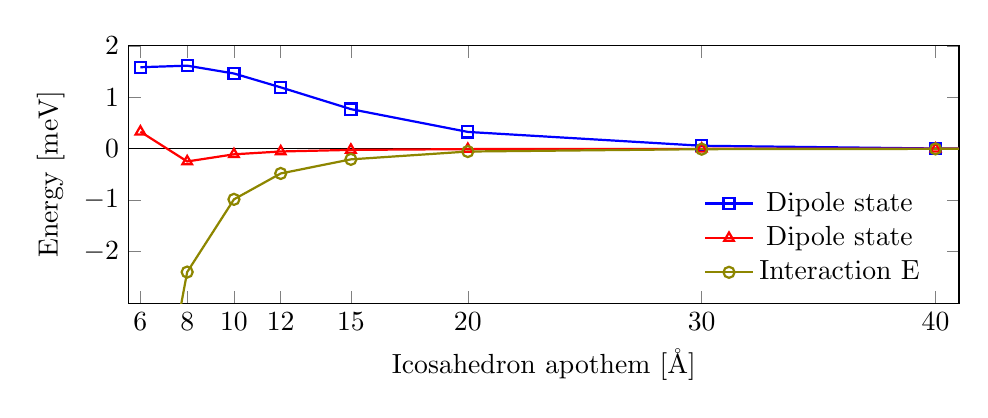
\begin{tikzpicture}
    \begin{axis}[
        width=1\textwidth,
        height=0.4\textwidth,
        ylabel={Energy [meV]},
        xlabel={Icosahedron apothem [\r{A}]},
        xmin=5.5, xmax=41,
        ymin=-3, ymax=2,
        xtick={6,8,10,12,15,20,30,40},
        ytick={0,-1, 1,-2,2},
        legend pos=south east,
        legend style={draw=none,fill=none}
    ]
    \draw ({rel axis cs:0,0}|-{axis cs:0,0}) -- ({rel axis cs:1,0}|-{axis cs:0,0});
    \draw ({rel axis cs:0,0}-|{axis cs:0,0}) -- ({rel axis cs:0,1}-|{axis cs:0,0});

    \addplot[
    color=blue,
    mark=square,
    line width=0.8pt
    ]
    coordinates {
        (6,1.584) (8,1.614) (10,1.462) (12,1.193) 
        (15,0.770) (20,0.327) (30,0.058) (40,0.005) (50,0.000)
    };
    \addlegendentry{Dipole state}

    \addplot[
        color=red,
        mark=triangle,
        line width=0.8pt
    ]
    coordinates {
        (6,0.331) (8,-0.247) (10,-0.108) (12,-0.053) 
        (15,-0.022) (20,-0.007) (30,-0.002) (40,-0.001) (50,0.000)
    };
    \addlegendentry{Dipole state}

    \addplot[
        color=olive,
        mark=o,
        line width=0.8pt
    ]
    coordinates {
        (6,-7.255) (8,-2.396) (10,-0.983) (12,-0.480) 
        (15,-0.206) (20,-0.054) (30,-0.008) (40,-0.002) (50,0.000)
    };
    \addlegendentry{Interaction E}
    \end{axis}
    \end{tikzpicture}